\documentclass[brudnopis]{xmgr}

% \documentclass[openright]{xmgr}

\usepackage{minted}

%\defaultfontfeatures{Scale=MatchLowercase}
%\setmainfont[Numbers=OldStyle,Ligatures=TeX]{Minion Pro}
%\setsansfont[Numbers=OldStyle,Ligatures=TeX]{Myriad Pro}
% for fontspec version < 2.0
% \setmainfont[Numbers=OldStyle,Mapping=tex-text]{Minion Pro}
% \setsansfont[Numbers=OldStyle,Mapping=tex-text]{Myriad Pro}
%\setmonofont[Scale=0.75]{Monaco}

% Opcjonalnie identyfikator dokumentu
% drukowany tylko z włączoną opcją 'brudnopis':
\wersja   {wersja wstępna [\ymdtoday]}

\author   {Krzysztof Sazon}
\nralbumu {243\,696}
\email    {krzysztof.sazon@protonmail.com}

\title    {Zastosowanie modelu szeregowania zadań częściowo zależnych w systemie otwartym w harmonogramowaniu danych tabelarycznych}
\date     {2020}
\miejsce  {Gdańsk}

\opiekun  {dr Hanna Furmańczyk}

% dodatkowe polecenia
%\renewcommand{\filename}[1]{\texttt{#1}}
%\definecolor{stress}{cmyk}{0,1,0.13,0} % RubineRed
%\definecolor{topic}{cmyk}{0.98,0.13,0,0.43} % MidnightBlue

\begin{document}

% streszczenie
\begin{abstract}
W pracy przedstawiono propozycję systemu szeregowania zadań na tabelarycznych zestawach danych w systemie komputerowym, opartą o model nazwany w literaturze "szeregowanie zadań częściowo zależnych w systemie otwartym" - \emph{Partially Concurrent Open Shop Schedule}  \emph{(PCOSS)}.\\
Przeanalizowano również jak wydajne pod kątem czasu przygotowania szeregowania są heurystyki opisane w literaturze.\\
\end{abstract}

% słowa kluczowe
\keywords{
partially concurrent open shop schedule,
tabular data,
csv,
pandas
}

% tytuł i spis treści
\maketitle

% wstęp
\introduction

W obecnych czasach wytwarzane są niespotykane do tej pory ilości danych (w latach 2017-2018 powstało 90\% danych powstałych od początku ludzkości do maja 2018 \cite{Forbes:2018:FBS}).
Nie istnieją też żadne przesłanki stanowiące o tym, że tempo wzrostu opadnie.
Dane te pozwalają na nowe podejścia do wglądu w zjawiska, które do tej pory były niemożliwe.
Jednocześnie prędkości przetwarzania komputerów nie rosną współmiernie do ilości tych danych. Jeszcze do niedawna trend wzrostu wydajności dostatecznie dobrze pokrywało tak zwane prawo Moore-a: ilość tranzystorów w układach zespolonych podwaja się co dwa lata \cite{MOORE:1965:X}. Poprzez miniaturyzację układów scalonych, procesy produkcyjne stają się coraz bardziej skomplikowane i wiele osób widzi perspektywę spowolnienia tego przyrostu \cite{NOTMOORE:2020:X}. Pozostawia to deficyt technologiczny, do pokrycia którego potrzebne są rozwiązania związane z oprogramowaniem, w szczególności rozwiązania algorytmiczne.
\medskip

W pracy zaproponowano rozwiązanie mogące przyspieszyć bardzo powszechne operacje na danych w postaci tabel.
\medskip

Przykładami danych tego typu są table w programie \emph{Microsoft Excel} i jemu podobnych, pliki z wartościami rozdzielanymi przecinkiem (\emph{Comma Separated Values} - \emph{CSV}), tabele i widoki w relacyjnych bazach danych, pliki \emph{Parquet} czy struktury tworzone przez biblioteki do manipulowania i analizy danych jak \emph{pandas}.
Można za ich pomocą reprezentować informacje z szerokiego spektrum dziedzin. Należą do nich między innymi dane pogodowe, wyniki giełdy, opisy przypadków osób z chorobami serca czy dzienniki połączeń sieciowych do danego serwera (tzw. \emph{logi}).

\chapter{Pochodzenie modelu szeregowania zadań częściowo zależnych w systemie otwartym i dotychczasowa literatura}
\chaptermark{Pochodzenie i dotychczasowa literatura}

\section{Początki szeregowania}
Szeregowanie towarzyszyło ludzkości od bardzo dawna, jednak początków współczesnego szeregowania można szukać we wprowadzeniu produkcji taśmowej w fabrykach Forda. Natomiast w matematycznym sensie za punkt otwierający ten rozdział można uznać algorytm Jacksona powstały na potrzeby przemysłu w latach pięćdziesiątych dwudziestego wieku (rozwiązanie w czasie wielomianowym problemu szeregowania w systemie ogólnym, w środowisku dwu maszynowym, z maksymalnie dwiema operacjami na zadanie) \cite{jackson1956extension}.
\medskip

\section{Szeregowanie}
Szeregowanie w szerokim sensie można opisać jako alokację zasobów do zadań na w pewnej przestrzeni czasu tak, aby alokacja możliwie najlepiej spełniała zadane kryterium optymalizacyjne, czyli zminimalizowany zostały koszt uszeregowania (lista kilka najbardziej powszechnych kryteriów optymalizacyjnych znajduje się w tym rozdziale). Powstało wiele prac na ten temat, z których cześć została zebrana w publikacjach \cite{graves1981review}, \cite{lawler1993sequencing} oraz \cite{lee1997current}.
\medskip

Formalne ujęcie problemu to:\\
% Posiadając zbiór maszyn $M=\{1,...,m\}$, które mają wykonywać operacje na zbiorze zadań $J=\{1,...,n\}$, szeregowaniem dla każdego zadania nazywamy alokacje jednego lub więcej interwałów czasu do jednej lub więcej maszyn \cite{brucker1999scheduling}.
% \medskip

Mamy zbiór $n$ zadań $\{i = 1,...,n\}$ i zbiór $m$ maszyn $\{M_1,...,M_m\}$. Każde zadanie $i$ składa się ze zbioru operacji $O_{ij} (j=1,...,n_i)$ z czasami przetwarzania $p_{ij}$. Każda operacja $O_{ij}$ musi być wykonana na maszynie $\mu_{ij} \in \{M_1,...,M_m\}$. Mogą istnieć relacje poprzedzania pomiędzy operacjami wszystkich zadań. Każde zadania może być wykonywane przez wyłącznie jedną maszynę naraz i każda maszyna może wykonywać co najwyżej jedną operację w danym momencie czasu. Celem jest znalezienie wykonalnego szeregowania które minimalizuje zadaną funkcję celu \cite{brucker1999scheduling}. Problem nazywamy deterministycznym, jeżeli wszystkie dane znane są stałe i z góry znane.
\medskip

Spośród dwu najważniejszych grup modeli szeregowania - szeregowanie na maszynach dedykowanych (\emph{Shop Scheduling}) oraz szeregowanie na maszynach równoległych (\emph{Parallel Processing Scheduling}) - opis którego znajdziemy między innymi w pracy \cite{drozdowski2009scheduling}, problem przedstawiony w tej pracy jest podproblemem tej pierwszej grupy. Grupa ta jest często wykorzystywana przy modelowaniu zjawisk takich jak działanie fabryk, warsztatów czy sieci komputerowych.
Opiera się na założeniu, że zadanie składa się z operacji, a każda operacja ma swój czas wykonywania i maszynę, na której powinna być wykonywana (w odróżnieniu od maszyn równoległych, gdzie każda maszyna może obsłużyć każdą operację).
\medskip

Wejściem dla tego problemu jest zbiór zadań, środowisko maszynowe, czasy wykonywania operacji na poszczególnych maszynach oraz zbiór ograniczeń.
Natomiast rozwiązaniem jest uszeregowanie operacji, czyli przypisanie każdej z nich czasu rozpoczęcia (równoważnie - czasu jej zakończenia).\\

Do opisu problemu szeregowania na maszynach dedykowanych w pracy \cite{graham1979optimization} wprowadzona została notacja trójpolowa ($\alpha|\beta|\gamma$), która opisuje środowisko maszynowe (pole $\alpha$), opis zbioru zadań (pole $\beta$) oraz funkcję kryterium optymalizacyjnego - funkcji, której wartość należy zoptymalizować (pole $\gamma$).\\

Najczęstsze wartości występujące w polach notacji dla procesorów dedykowanych:\\

Dla pola $\alpha$:
\begin{itemize}
    % \item $P$ - procesory identyczne
    % \item $Q$ - procesory jednorodne
    % \item $R$ - procesory dowolne
    \item $O$ - system otwarty
    \item $F$ - system przepływowy
    \item $J$ - system ogólny
\end{itemize}

Dla pola $\beta$:
\begin{itemize}
    \item pole puste - zadania są niepodzielne, niezależne, z $r_j=0$, czasy wykonania i ewentualne terminy zakończenia $d_j$ dowolne
    \item $pmtn$ - zadania podzielne
    \item $prec$ - zadania zależne
    \item $r_j$ - różne wartości momentów przybycia
    % \item $p_j=1$ lub $UET$ - operacje jednostkowe
    \item $p_{ij}\in\{0,1\}$ - operacje jednostkowe lub puste
    \item $C_j\leq d_j$ - istnieją wymagane i nieprzekraczalne terminy zakończenia zadań
    \item $no\-idle$ - procesory muszą pracować w sposób ciągły, bez okienek
    \item $no\-wait$ - okienka między operacjami w zadaniach są zabronione
    \item $in-tree, out-tree, chains$ - różne szczególne postaci relacji zależności kolejnościowych
\end{itemize}

Oraz dla pola $\gamma$:
\begin{itemize}
    \item $C_{max}$ - długość uszeregowania
    \item $\sum{C_k}$ - całkowity (łączny) czas zakończenia zadań
    \item $\bar{F}$ - średni czas przepływu
\end{itemize}
% job shop to szeregowanie w systemie ogólnym lub gniazdowym
% flow shop - to szeregowanie w systemie przepływowym
% open shop - system otwarty.
% shop schdule - szeregowanie na maszynach dedykowanych

% System gniazdowy
% 	W systemie gniazdowym (ogólnym) kolej-ność maszyn mających wykonać operacje jest różna, ale ściśle określona dla każdego zadania (zadania mogą mieć różną ilość operacji). 

Do głównych modeli szeregowania na maszynach dedykowanych należą:
\begin{itemize}
    \item szeregowanie w systemie ogólnym (gniazdowym, \emph{Job Shop Scheduling}), w którym operacje wykonywane są liniowo, zgodnie z zadaną kolejnością, niekoniecznie tą samą dla wszystkich zadań
    \item szeregowanie w systemie przepływowym (\emph{Flow Shop Scheduling}), w którym operacje wykonywane są liniowo, zgodnie z zadaną kolejnością a każde zadanie ma tę samą kolejność
    \item system otwarty (\emph{Open Shop Scheduling}), w którym operacje na danym zadaniu mogą być wykonywane w dowolnej kolejności
\end{itemize}

\section{Model szeregowania w systemie otwartym}
\medskip

Powstały w latach siedemdziesiątych model szeregowania w systemie otwartym (\emph{Open Shop Schedule} - \emph{OSS}) to sposób szeregowania zadań, gdzie kolejność wykonywania operacji nie wpływa na wynik całego rozkładu. Jego klasyczna definicja to:
\medskip

Istnieje zbiór $N=\{1,...,n\}$ zadań, z których każde posiada zbiór operacji, które muszą być wykonywane na zbiorze różnych maszyn $M=\{1,...,m\}$. Operacja wykonania zadnia $j$ na maszynie $i$ jest oznaczona jako $O_{ij}$, a czas jej wykonywania jako $p_{ij}$.
% Jeżeli zadanie $j$ posiada czas dostępu (czyli termin od którego może zostać podjęte) oraz termin ukończenia, oznaczamy je odpowiednio przez $r_j$ i $d_j$.
Kolejność wykonywania zadań jest niematerialna, czyli nie ma wpływu na wynik rozkładu. Każda maszyna może wykonywać co najwyżej jedną operację na raz. Celem jest ustalenie rozkładu (czyli przypisanie każdej operacji czasu jej rozpoczęcia lub zakończenia), w taki sposób, że zadane kryterium optymalizacyjne jest osiągnięte. \cite{ahmadian2020four}.
\medskip

\section{Model szeregowania zadań częściowo zależnych w systemie otwartym}
Model szeregowania zadań częściowo zależnych w systemie otwartym (\emph{Partially Concurrent Open Shop Schedule - PCOSS}), na którym skupia się niniejsza praca, został wprowadzony w 2014 roku przez Tal Grinshpoun, Hagai Ilani i Elad Shufan w pracy \emph{Partially-Concurrent Open Shop Scheduling} \cite{grinshpoun2014partially} jako generalizacja modelu szeregowania w systemie otwartym (\emph{OSS}).\\
\medskip

Model \emph{PCOSS} względem \emph{OSS} wprowadza możliwość równoczesnego wykonywania niektórych operacji. Motywacją dla pracy był problem stworzenia rozkładu pracy dla techników sprawdzających samoloty w hangarze, gdzie część czynności może być wykonywana równolegle, a inne nie mogą odbywać się jednocześnie.

\section{Inne modele skojarzone z modelowaniem w systemie otwartym}
Istnieją różne generalizacje modelowania w systemie otwartym oraz modele, w których łączy się go z innymi typami szeregowania na maszynach dedykowanych.
Jako przykład generalizacji można podać \emph{Multiprocessor Open Shop Schedule}, w którym kilka identycznych maszyn może pracować równolegle nad jedną operacją \cite{adakmultiprocessor}, oraz \emph{Concurrent Open Shop Schedule}, który jest szczególnym przypadkiem \emph{PCOSS}, w którym wszystkie maszyny mogą operować na zadaniu równolegle. \cite{wagneur1993openshops}.
Łączeniem \emph{OSS} z innymi modelami jest \emph{Mixed Shop Schedule}, w którym zadania mogą przechodzić przez system ogólny, system przepływowy, system otwarty, oraz różne ich kombinacje.

\section{Dotychczasowa literatura o szeregowaniu zadań częściowo zależnych w systemie otwartym}
W dziedzinie badań związanych z szeregowania zadań częściowo zależnych w systemie otwartym przewijają się głównie nazwiska badaczy z \emph{Ariel University} w Izraelu: Tal Grinshpoun, Hagai Ilani i Elad Shufan. Pracę \cite{grinshpoun2014partially} zaprezentowali oni na \emph{10th International Conference on the Practice And Theory of Automated Timetabling (PATAT 2014)}. Motywacją dla tej pracy był problem przydzielania techników do obsługi floty samolotów (sprawdzenia ich przed lotem). Problem jest podobny do standardowego systemu otwartego pod kątem braku wpływu kolejności wykonywania badań na efekt końcowy (decyzje czy samolot ma wszystkie podzespoły sprawne). W celu skrócenia czasu cześć operacji można wykonywać jednocześnie, co w pewnym stopniu upodabnia sytuację do tej modelowanej przez \emph{Multiprocessor Open Shop Schedule}, opisywanej między innymi w pracy \cite{adakmultiprocessor}. Problemem w tym modelu są jednakże operacje na jednym samolocie, które wzajemnie się wykluczają, na przykład poprzez zakłócanie odczytów narzędzi pomiarowych przez inne procesy. Operacje te są reprezentowane przez graf konfliktu, będący jedną z danych wejściowych dla modelu. W rzeczy samej, system otwarty oraz \emph{Multiprocessor Open Shop Schedule} są skrajnymi przypadkami szeregowania zadań częściowo zależnych w systemie otwartym - odpowiednio z grafem konfliktu, który ma wszystkie krawędzie poza tymi między różnymi maszynami a zadaniami oraz z grafem konfliktu, który ma krawędzie wyłącznie pomiędzy różnymi zadaniami w obrębie jednej maszyny.\\
Autorzy proponują przestawienie rozkładu jako macierz rang (\emph{Rank Matrix}) $A = (a_{ij})$, gdzie wartość komórki $a_{ij} = k$ oznacza, że ścieżka prowadząca do operacji $(i, j)$ z maksymalną ilością operacji ma $k$ operacji \cite{brasel2008heuristic}. Macierz ta ma przełożenie 1:1 na znajomość czasów rozpoczęcia każdej z operacji (lub równoważnie jej zakończenia) - sposób konstrukcji oraz obliczania uszeregowania znajduje się w tejże pracy. Zaproponowano użycie następującej notacji trójpolowej dla \emph{PCOSS}: $O|pconc|f_n$, gdzie $f_n$ jest kryterium optymalizacyjnym. Autorzy wskazują na to, że problem sprowadza się do orientowaniem grafu konfliktu tak, żeby był acykliczny i najdłuższa ścieżka w nim była możliwie najkrótsza. Pokazane zostaje, że problem jest NP-trudny już dla pojedynczego zadania i jednostkowych czasów, z czego wynika, że ogólny przypadek jest również NP-trudny. Jako heurystykę konstrukcyjną autorzy podają adaptację algorytmu wstawiania z zastosowaniem szukania wiązkowego (\emph{insertion with beam search}), prezentowanego między innymi w pracy \cite{brasel1993constructive}.
\medskip

W pracy \cite{ilani2016partially} ci sami autorzy opisują relację między szczególnymi przypadkami \emph{PCOSS} a technikami stosowanymi przy kolorowaniu grafów. Prfaca zawiera interesujące sposoby podejścia do zagadnienia, które jednakowoż nie mają oczywistych zastosowań w tematyce niniejszej pracy, gdyż skupiają się na modelach z wywłaszczaniem, wersjach \emph{uniform} (wszystkie zadania mają jednakowe czasy wykonywania na poszczególnych maszynach) oraz takich z czasami jednostkowymi (wszystkie operacja trwają jedną jednostkę czasu) problemu \emph{PCOSS}. Autorzy wskazują między innymi na możliwość przygotowania uszeregowania dla wersji \emph{PCOSS} z wywłaszczeniami w czasach całkowitych (\emph{integral-preemption PCOSS} w czasie wielomianowym względem rozmiaru wejścia dla niektórych przypadków grafu konfliktu - gdy jest on grafem doskonałym. Graf doskonały to graf, którego liczba chromatyczna każdego podgrafu indukowanego wierzchołkowo równa jest rozmiarowi największej kliki tego podgrafu \cite{diestel2010graph}. Bazują przy tym na wynikach pracy \cite{grotschel1984polynomial}, gdzie wykazane zostaje, że każdy graf doskonały może zostać polokorowany w czasie wielomianowym.
\medskip

Praca \cite{ilani2018partially} autorstwa Tal Grinshpoun, Hagai Ilani i Elad Shufan wprowadza kolejne zagadnienie do tematyki \emph{PCOSS}: ograniczenie zasobów. Ograniczone zasoby, w rozumieniu tej pracy, to zasoby, z których mogą korzystać maszyny wspólnie, i których liczbę ogranicza ilość operacji, które mogą być wykonywanie jednocześnie. Po raz kolejny twórcy pracy sięgają do wykorzystania kolorowania grafów, jako środka metody projekcji problemu. W pracy wykorzystane są badania problemu znanego w literaturze pod nazwą ograniczonego kolorowania wierzchołkowego (\emph{Bounded Vertex Colouring}) - kolorowania, w którym każdy kolor wykorzystywany jest maksymalnie pewną ustaloną liczę razy \cite{hansen1993bounded}.

\section{Oznaczenia przyjęte w pracy}

Hasła \emph{tabela} i \emph{tablica} stosowane będą zamiennie i będą oznaczały strukturę danych składającą się z listy krotek. 
\medskip

W celu uniknięcia dwuznaczności słowa \emph{procesor} w pracy tratującej zarówno o modelu matematycznym jak i o systemach komputerowych przyjęto używanie go w rozumieniu pochodzącym z modelu matematycznego (inaczej \emph{maszyna}).
\emph{Procesor} w rozumieniu układu scalonego w systemie komputerowym będzie oznaczany anglojęzycznym skrótem, takim jak \emph{CPU} (\emph{Central Processing Unit}) czy \emph{GPU} (\emph{Graphics Processing Unit}).
\medskip

Hasłem \emph{komórka} oznaczony zostanie konkretny, identyfikowalny za pomocą indeksu wiersza i kolumny element tabeli.

\chapter{Dane tabelaryczne}

Dane tabelarycznie w postaci elektronicznej są w dzisiejszych czasach codziennym elementem pracy wielu osób, zarówno w środowiskach naukowych jak i w świecie konsumenckim i przemysłowym. Jest to jeden z najbardziej powszechnych sposobów reprezentacji zbiorów danych. Przykładami dziedzin, gdzie są one szczególnie istotne mogą być: analiza statystyczna, handel, magazynowanie, prognozowanie trendów czy systemy, które na bazie bodźców ze środowiska modyfikują swoje działanie.
\medskip

Słownik \emph{Merriam-Webster} definiuje "tabelaryczny" jako "osadzony w wierszach i kolumnach" \cite{MW:TAB}
\medskip

Moduł języka \emph{Python} - \emph{pandas} definiuje "DataFrame" jako "dwuwymiarowe, potencjalnie heterogeniczne dane tabelaryczne" \cite{P:DF}.
\medskip

Baza danych \emph{Postgres} definiuje "tabelę" jako "kolekcję krotek mających wspólną strukturę danych (ta sama ilość atrybutów, w tej samej kolejności mających tę samą nazwę i typ per pozycja)" \cite{PSQL:TAB}.
\medskip

System opisany w tej pracy może być zastosowany do danych, które mogą być opisane przez każdą z tych definicji z osobna.

\chapter{Zastosowanie modelu PCOSS do danych tabelarycznych}
\chaptermark{Zastosowanie do danych tabelarycznych}

Praca skupia się na takich sytuacjach, gdy sekwencyjne lub naiwnie zrównolegnione wykonywanie operacji zajmuje zbyt wiele czasu lub jest niemożliwe z uwagi na ograniczenia narzucone na wykonywanie operacji na tabeli.
Ograniczenia te odpowiadają grafowi konfliktu w \emph{PCOSS}.
\medskip

Źródła tych ograniczeń można podzielić na trzy kategorie:
\begin{enumerate}
    \item skutkujące niepotrzebnie wysokim wykorzystaniem zasobów,
    \item takie gdzie zrównolegnianie prowadzi do pogorszenia wartości funkcji optymalizacji (pogorszenie wydajności),
    \item takie, gdzie wykonywanie par operacji na jednym wierszu może prowadzić do nieprawidłowych wyników.
\end{enumerate}
\medskip

Przykłady
\begin{enumerate}
    \item korzystając z różnych połączeń z serwerem per różne wiersze, niekorzystne może być zlecenie przeliczenia wartości z dwu kolumn naraz na tym samym serwerze (przełączanie kontekstów procesora, odczyt z \emph{HDD} po stronie serwera etc.),
    \item zapisując wyniki do różnych baz SQLite per różne wiersze, jednoczesny zapis wartości obliczanej na dwu kolumnach do jednej bazy spowoduje zablokowanie zapisu drugiego wyniku, do czasu skończenia zapisu pierwszego,
    \item zależności między danymi w różnych kolumnach tego samego wiersza; mając wiersze z kolumnami wskazującymi na siebie, nie powinniśmy jednocześnie zmieniać wartości obydwu tych kolumn, gdyż może to prowadzić to niespójności danych.
\end{enumerate}
\medskip

Podobne rozumowanie, w szczególności w odniesieniu do nawiązywania połączeń między różnymi serwerami można przeprowadzić dla grafu konfliktu między różnymi wierszami tej samej kolumny oraz dowolnymi parami komórek.
\medskip

Warto zauważyć, że powyższe problemy mają względnie nieduże znaczenie w większości przypadków, gdy cały rozkład wykonywany jest na jednej maszynie lub przy niedużych ilościach danych. Można je wtedy rozwiązać między innymi za pomocą odpowiednich mechanizmów blokowania dostępu do zasobów (\emph{locking}).
Sytuacja zmienia się gdy musimy przetworzyć duże ilości danych na systemach rozproszonych.
\medskip

Zastosowanie proponowanego frameworku w macierzach FPGA, sieciach procesorów oraz w przypadku korzystania z sieciowych interfejsów do przetwarzania danych wydaje się być bardziej racjonalne i pożądane niż zastosowanie go dla pojedynczej maszyny.

\chapter{Relacja między modelem matematycznym a architekturą systemu}

Przy przyjętych w poprzednim rozdziale założeniach rolę \emph{procesorów} z modelu matematycznego przejmują urządzenia (lub ich systemy), takie jak \emph{API} serwerów sieciowych, \emph{CPU}, \emph{GPU} czy dyski twarde.
\medskip

\emph{Zadania} interpretowane są jako kolejne wiersze lub ich agregaty.
\medskip

Z powyższego wynika bezpośrednio, że \emph{operacją} staje się praca pewnej instancji pewnego systemu (\emph{procesora} w rozumieniu wynikającym z modelu matematycznego) na konkretnym zbiorze wierszy.
\medskip

W szczególnym (a zarazem najczęstszym przypadku) zestaw wierszy zawiera jeden wiersz, a zestaw kolumn zawiera jedną kolumnę, co implikuje traktowanie komórki jako operacji.
\medskip

Po ewentualnej agregacji kolumn i wierszy powstała tabela przestawiać będzie zestaw zadań (danych) w wierszach, maszyn (urządzeń) w kolumnach i operacje (przetwarzanie danych przez maszynę) w komórkach.

\chapter{Typ danych analizowany w pracy}

Sposób działania systemu jest w dużej mierze niezależny od danych wejściowych - warunkiem jest reprezentowane ich w postaci tabeli z zadaniami w wierszach i maszynami w kolumnach.
Mogą więc być to na przykład dane tekstowe, liczbowe, obiekty, adresy serwisów internetowych, obrazy, pliki czy też referencje do innych tabel.
\medskip

W pracy pominięto aspekt zbierania danych jako niezwiązany bezpośrednio z szeregowaniem operacji na nich.
\medskip

W celu uzyskania oczekiwanych informacji z zestawu danych należy je odpowiednio spreparować a następnie uruchomić narzędzia analityczne na nich.
\medskip

Wprowadzimy abstrakcję, gdzie w wypadku operacji agregowania określone na wejściu zestawy agregowanych kolumn traktowane będą jako pojedyncze kolumny, a określone na wejściu zestawy agregowanych wierszy - jako pojedyncze wiersze.

Dzięki tej abstrakcji możemy uprościć rozważania, nie tracąc zarazem poprawności działania.

\section{Kreacja danych testowych}

Danymi testowymi będzie lista $n$ krotek o rozmiarze $m$ elementów każda.
Każda kolejna krotka będzie traktowana jako nowy wiersz, natomiast wszystkie indeksy krotek będą odpowiadały kolumnom. 
\medskip

Taki zestaw danych przekłada się na wiele modeli wykorzystywanych w komputerowej analizie danych, jak na przykład tabele czy widoki w relacyjnych bazach danych, \emph{DataFrame} w pythonowym pakiecie \emph{pandas} czy dwuwymiarowa macierz w \emph{numpy}.
\medskip
Relacyjne bazy danych to sposoby reprezentacji i przechowywania zbiorów danych oparte o idee zaproponowane przez Edgara Codda, około roku 1970. Relacyjne bazy dane organizują dane w tabelach, które składają się z wierszy (rekordów, krotek) i kolumn (pól, atrybutów). Table posiadają relacje (związki) między sobą, pozwalające na efektywne wykorzystanie zasobów. Językiem programowania najczęściej stosowanym do operacji na bazach danych są różne wariacje \emph{Structured Query Language} - \emph{SQL} \cite{RDB1:2020:X}\cite{RDB2:2020:X}\cite{RDB3:2010:X}.

\emph{pandas} to stosowana w języku python biblioteka złożonych struktur i narzędzi do pracy ze zbiorami danymi strukturalnymi powszechnie wykorzystywanych w statystyce, finansach, naukach społecznych i na wielu innych polach. Biblioteka dostarcza zintegrowane, intuicyjne narzędzia do wykonywania powszechnych manipulacji danych i ich analizy. Służy ona jako silny dodatek do istniejących narzędzi w języku python, jednocześnie implementując i rozwijając narzędzia manipulacji danymi obecne w innych językach zorientowanych na programowanie statystyczne, takich jak R \cite{PANDAS1:2011:X}\cite{PANDAS2:2020:X}.

\emph{numpy} to również stosowana w języku python biblioteka, która jest zestawem rozszerzeń do niego, pozwalającym na efektywne manipulowanie dużymi zbiorami danych zorganizowanymi w krato-podobny sposób oraz przeprowadzanie obliczeń numerycznych \cite{NUMPY1:2020:X}\cite{NUMPY2:1999:X}.
\medskip

W rzeczywistym zastosowaniu komórki będą zawierały dane podlegające odpowiednim procesom (obliczeniom).
W danych testowych będą liczbami losowymi, reprezentującymi rozmiar wejścia do funkcji, która ma wykonać obliczenia na nich.
\medskip

\begin{table}[!tbh]
\begin{tabular}{|l|l|l|l|l|l|} \hline
$r / col$   & $c_1$     & $c_2$     & ...   & $c_{m-1}$ & $c_{m}$   \\ \hline
$r_1$       & $2562$    & $45656$   & ...   & $54656$   & $0$       \\ \hline
$r_2$       & $4546$    & $0$       & ...   & $7861$    & $12135$   \\ \hline
$...$       & $...$     & $...$     & $...$ & $...$     & $...$     \\ \hline
$r_{n-1}$   & $2541$   & $712$      & ...   & $3574$    & $9347$    \\ \hline
$r_{n}$     & $4561$   & $4214$     & ...   & $9753$    & $4125$    \\ \hline
\end{tabular}
\caption{Przykład danych testowych\label{tab:example-sched-out}}
\source{Własne}
\end{table}

\chapter{Algorytm działania dyspozytora}

\section{Wstęp}

W rozumieniu tej pracy \emph{dyspozytor} to system mający na celu poprawne (wykonalne i zgodne z ograniczeniami) zaszeregowanie i rozdzielanie zadań pomiędzy pomiędzy dostępne procesory.
\medskip

Wysokopoziomowo algorytm działania dyspozytora opierał będzie się o następujące kroki

\begin{enumerate}
    \item pobranie danych, ustawienie wartości domyślnych
    \item grupowanie danych
    \item przydzielenie szacunkowych czasów wykonania poszczególnych operacji
    \item dobór algorytmu szeregowania 
    \item przygotowanie uszeregowania
    \item czuwanie nad prawidłowym wykonaniem uszeregowania
\end{enumerate}

Każdy z powyższych kroków szczegółowo opisany jest w tym rozdziale.
\newpage

\section{Pobranie danych, ustawienie wartości domyślnych}

Na wejściu algorytm otrzymuje następujące dane wejściowe

\begin{enumerate}
    \item tabelę w wybranej reprezentacji
    \item funkcję grupowania wierszy (argument opcjonalny)
    \item funkcję grupowania kolumn (argument opcjonalny)
    \item listę operacji do wykonania na tabeli
    \item graf konfliktu (argument opcjonalny)
    \item tabelę złożoności obliczeniowej (zgrupowanych) kolumn (argument opcjonalny)
    \item tabelę czasów przetwarzania (zgrupowanych) kolumn (argument opcjonalny)
    \item algorytm szeregowania (argument opcjonalny)
    \item kryterium optymalizacyjne (argument opcjonalny)
\end{enumerate}

% \todo[inline]{dać przykład prawidłowego formatu każdego argumentu}

Tabela \ref{tab:args-default} zawiera domyślne wartości argumentów opcjonalnych
\medskip

% \todo{tak często się te nazwy przewijają, że być może warto nadać im symbole}

\begin{table}[!tbh]
\begin{tabular}{|l|l|l|} \hline
Idx. arg. & Wartość domyślna & Interpretacja wartości domyślnej \\ \hline
2 & funkcja identyczności   & brak grupowania wierszy \\ \hline
3 & funkcja identyczności   & brak grupowania kolumn \\ \hline
5 & graf pusty              & wszystkie operacje mogą być wykonywane jednocześnie \\ \hline
6 & nil                     & algorytm sam ustala złożoność \\ \hline
7 & nil                     & algorytm sam ustala czasy przetwarzania \\ \hline
8 & nil                     & algorytm sam dobiera algorytm \\ \hline
9 & $C_{max}$               & kryterium całkowitej długości uszeregowania \\ \hline
\end{tabular}
\caption{Domyślne wartości wejściowe algorytmu i ich interpretacja\label{tab:args-default}}
\source{Własne}
\end{table}
\medskip

Zagadnienie postępowania algorytmu w zależności od tego, które parametry zostały podane szerzej omówione zostanie w kolejnych podrozdziałach.

\section{Grupowanie danych}

W tej pracy agregacja rozumiana będzie jako proces łączenia kilku wartości w jedną reprezentatywną wartość.
\medskip

Logika działania agregacji na wierszach podąża za logiką przyjęta między innymi przez język \emph{SQL}, technologię \emph{LINQ} na platformie \emph{.Net} czy różne moduły języka \emph{Python}, w szczególności \emph{pandas}.
\medskip

Agregacja w zastosowaniach praktycznych jest jedną z podstawowych operacji przy przetwarzaniu danych, np. w celu ich analizy.
Pozwala ona łączyć duże ilości danych w logiczne grupy, które reprezentują analizowane właściwości tych danych.
\medskip

Agregację w takim rozumieniu można podzielić na dwa etapy:
\begin{itemize}
    \item grupowanie danych wg. funkcji grupującej
    \item wykonanie funkcji docelowej na zgrupowanych wartościach
\end{itemize}
\medskip

Przykład grupowania znajduje się poniżej.
\medskip

W przypadku, gdy podane są funkcje grupowania wierszy lub kolumn, algorytm tworzy zgrupowania zawierające indeksy zakresów zawieranych w tych zgrupowaniach, czyli łączy zestawy komórek w pojedyncze komórki na podstawie zadanego klucza (funkcji).
\medskip

Tak przygotowane dane gotowe są do przetwarzania w kolejnych etapach działania algorytmu.

\subsubsection{Przykład}
\medskip

Przygotowano tabelę wejściową \ref{tab:example-input}, w której znajdują się fikcyjne dane na temat sprzedaży produktów \emph{M1} i \emph{M2} na terenie trzech krajów w dwudniowym okienku czasowym.
\medskip

Dla tej tabeli przygotowane zostało takie zgrupowanie wierszy, że kluczem grupowania są jednakowe wartości w kolumnie \emph{Kraj} (funkcja \ref{eq:example-row-agg}).
\medskip

Dla kolumn przygotowane zostało takie zgrupowanie, że z kolumn \emph{Sprzedaż$\_$M1} i \emph{Sprzedaż$\_$M2} powstaje jedna kolumna \emph{Sprzedaż$\_$M1$\_$Sprzedaż$\_$M2} (funkcja \ref{eq:example-col-agg}).
\medskip

Po zastosowaniu funkcji sumy na zgrupowanych komórkach wynikowej kolumny należy to interpretować jako sumaryczną sprzedaż wszystkich produktów w całym okresie w danych krajach.

\begin{table}[!tbh]
\begin{tabular}{|l|l|l|l|l|} \hline
Indeks & Kraj & Data & Sprzedaż$\_$M1 & Sprzedaż$\_$M2 \\ \hline
1 & Polska & 01.01.2020 & 7 & 3 \\ \hline
2 & Niemcy & 01.01.2020 & 2 & 6 \\ \hline
3 & Rosja & 01.01.2020 & 5 & 1 \\ \hline
4 & Polska & 02.01.2020 & 2 & 6 \\ \hline
5 & Niemcy & 02.01.2020 & 4 & 2 \\ \hline
6 & Rosja & 02.01.2020 & 17 & 3 \\ \hline
\end{tabular}
\caption{Przykładowa tabela do zagregowania \label{tab:example-input}}
\source{Własne}
\end{table}
\medskip

Dla przejrzystości funkcji zastosowane zostały skróty
\medskip

\begin{itemize}
    \item Indeks - $i$
    \item Kraj - $k$
    \item Data - $d$
    \item Sprzedaż$\_$M1 - $s_{m1}$
    \item Sprzedaż$\_$M2 - $s_{m2}$
\end{itemize}
\medskip

Funkcja grupowania kolumn
\begin{equation} \label{eq:example-col-agg}
\lambda (i, k, d, s_{m1}, s_{m2}) \\ \Rightarrow (i, k, d, (s_{m1}, s_{m2}))
\end{equation}
\medskip

Funkcja grupowania wierszy
\begin{equation} \label{eq:example-row-agg}
\lambda (w_1, w_2, ..., w_{n-1}, w_n) \\ \Rightarrow (w_{g1}, w_{g2}, ..., w_{gm-1}, w_{gm}) 
\end{equation}
\medskip

gdzie $w_{gx}$ po prawej stronie transformacji, to grupa takich $w_y$ (po lewej stronie), dla których $k$ (kraj) to $x$
\medskip

Otrzymujemy tabelę wyjściową \ref{tab:example-output}, gotową do obróbki w następnym etapie.
Dla przejrzystości w komórkach nie znajdują się indeksy z tabeli wejściowej, tylko wartości kryjące się pod tymi indeksami.

\begin{table}[!tbh]
\begin{tabular}{|l|l|l|l|} \hline
Indeks & Kraj & Dzień & Sprzedaż$\_$M1$\_$Sprzedaż$\_$M2 \\ \hline
(1,4) & Polska & (01.01.2020, 02.01.2020) & ((7,3), (2,6)) \\ \hline
(2,5) & Niemcy & (01.01.2020, 02.01.2020) & ((2,6), (4,2)) \\ \hline
(3,6) & Rosja & (01.01.2020, 02.01.2020) & ((5,1), (17,3)) \\ \hline
\end{tabular}
\caption{Przykładowa tabela po grupowaniu\label{tab:example-output}}
\source{Własne}
\end{table}

\newpage

\section{Przydzielenie szacunkowych czasów wykonania poszczególnych operacji}

W celu przygotowania poprawnego rozkładu należy znać lub oszacować wartości czasów wykonywania poszczególnych operacji.\medskip

Z założeń podanie jednocześnie czasów w postaci argumentów "tabela złożoności obliczeniowej (zgrupowanych) kolumn" oraz "tabela czasów przetwarzania (zgrupowanych) kolumn" jest prawdopodobnie błędem ze strony użytkownika. W takim wypadku zostanie zgłoszony błąd i algorytm przerwie działanie.\medskip

Schemat działania przydzielania czasu został przedstawiony na diagramie \ref{diag:time-assign}.

\begin{figure}[!tbh]
\centering
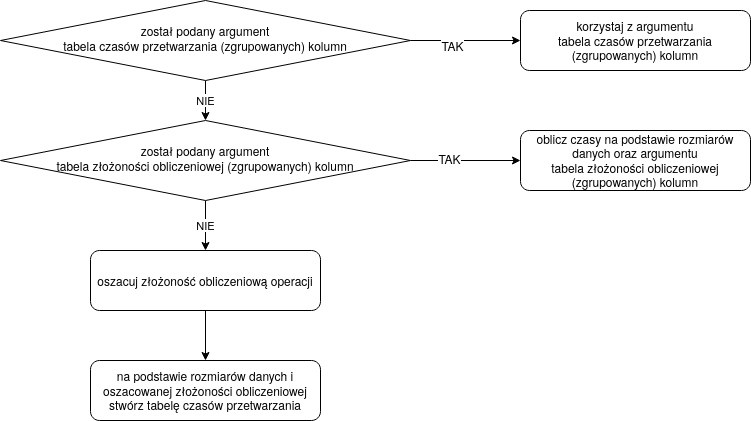
\includegraphics[width=.8\hsize]{fig/przydzielanie_czasow.png}
\caption{Schemat postępowania przy przydzielaniu czasu\label{diag:time-assign}}
\source{Opracowanie własne}
\end{figure}
\medskip

\subsubsection{Zachowanie algorytmu w zależności od podanych danych na temat czasu}

\myparagraph{Podano argument "tabela czasów przetwarzania (zgrupowanych) kolumn"}

W przypadku podania poprawnej macierzy czasów operacji ta część algorytmu nie jest wykonywana; zakładamy, że użytkownik podał prawidłowe wartości.
W szczególnym przypadku zadane mogą zostać jednakowe czasy wykonywania operacji.

\myparagraph{Podano argument "tabela złożoności obliczeniowej (zgrupowanych) kolumn"}

Ważnym aspektem tego argumentu, jest fakt, że w dziedzinie praktycznej podanie złożoności obliczeniowej nie może ograniczać się do podania samego asymptotycznego tempa wzrostu - $O(n)$; konieczne jest precyzyjniejsze oszacowanie, wraz ze współczynnikiem oraz czynnikiem dodanym (opóźnieniem, latencją).
\medskip

Jeżeli na wejściu do algorytmu znajduje się argument "tabela złożoności obliczeniowej (zgrupowanych) kolumn", jedyną operacją, która musi zostać wykonana jest podstawienie rozmiarów danych z poszczególnych komórek pod funkcje podane na wejściu.
\medskip

W szczególnym wypadku użytkownik może podać czasy niezależne od rozmiaru wejścia - na przykład czasy jednostkowe.
\medskip

\myparagraph{Nie podano żadnego z argumentów odnoszących się do czasów przetwarzania}

Na podstawie analizy kilku (np. losowych, lub pierwszych) (zgrupowanych) wierszy algorytm oszacuje złożoność operacji na danym procesorze.
W tym celu zostanie porównany rozmiar wejścia z czasem, w którym jest wykonywany, następnie wykorzystując funkcję \emph{curve\_fit} z pakietu \emph{scipy.optimize} zostaną dobrane parametry $a$, $b$, $c$ do funkcji

$$t = f(b * s^a + c)$$

Gdzie $t$ to czas wykonywania, a $s$ to rozmiar danych.
\medskip

Funkcja \emph{curve\_fit} działa wykorzystując metodą najmniejszych kwadratów korzystając z zadanego algorytmu, np Levenberga-Marquardta \cite{lourakis2005brief}.
\medskip

Problem niepokrycia wszystkich możliwych funkcji czasów przetwarzania poruszony został w rozdziale \ref{chap:extend}.

% \todo[inline]{być może łatwiej będzie skorzystać z cProfile}
% \todo[inline]{napisać to matematycznie}
% \todo[inline]{opisać w jaki sposób oceniana jest złożoność funkcji przez curve\_fit}

\section{Dobór algorytmu szeregowania}

% \todo[inline]{być może to dobieranie nic ciekawego nie wnosi - seria if-ów}

Jeżeli użytkownik poda obsługiwany przez program algorytm szeregowania, program wykorzysta swoją implementację tego algorytmu.
W przypadku niezaimplementowania wymaganego przez użytkownika algorytmu szeregowania program zgłosi błąd.
\medskip

Jeżeli algorytm szeregowania nie zostanie podany, to przy zadanym kryterium optymalizacyjnym program dobierze odpowiedni algorytm szeregowania służący do przygotowania optymalnego rozkładu.
\medskip

Dobór algorytmu polegał będzie na poruszaniu się po drzewie decyzji (bez ingerencji użytkownika).
Wybór podjęty przez rozwiązanie funkcji zwracającej \emph{prawda/fałsz} na każdym poziomu prowadził będzie do kolejnej funkcji w drzewie lub na poziomie liścia - do konkretnego algorytmu.

\section{Przygotowanie uszeregowania}

Po rozważeniu dwu metod możliwości rozdysponowania operacji pomiędzy procesory: z egzekutorem (koordynatorem) oraz w bez (w sposób nieskoordynowany) wybrana została metoda uwzględniająca egzekutora.
\medskip

Mimo większej prostoty mechanizmu gdzie każdemu procesorowi zadana jest seria operacji do wykonania w określonych czasach, mechanizm z koordynatorem jest bardziej odporny na błędy i oferuje możliwość łatwiejszej rozbudowy.

Gdy przygotowane zostaną

\begin{itemize}
    \item tabela wejściową z punkcie "Pobranie i preparacja danych"
    \item tabela czasów z punktu "Przydzielenie szacunkowych czasów wykonania poszczególnych operacji"
    \item graf konfliktu z wejścia
    \item algorytm szeregowania z punktu "Dobór algorytmu szeregowania"
\end{itemize}

można przystąpić do konstrukcji uszeregowania.
\medskip

Konstrukcja uszeregowania polega na wykonaniu danego algorytmu szeregowania z danymi wejściowymi.
\medskip

Finalny rozkład zostanie przedstawiony w formie tabeli, której indeksy wierszy ($t_i$) będą zawierały informacje o planowanym czasie rozpoczęcia wykonania operacji, kolumny ($p_j$) przedstawiają procesory natomiast w komórce (koleje małe litery alfabetu) znajduje indeks wiersz i kolumny zagregowanej tabeli wejściowej (lokalizacja komórki) w postaci dwójki [indeks wiersza, indeks kolumny].
% \todo{matematycznie zapisać}
\medskip

Przykładowy rozkład wynikowy został przedstawiony w tabeli \ref{tab:example-sched-out}.
\medskip

Należy zauważyć, że taki rozkład jest transponowanym klasycznym wykresem Gantta z dyskretnymi czasami rozpoczynania zadań.

\begin{table}[!tbh]
\begin{tabular}{|l|l|l|l|l|l|} \hline
Czas / proc & $p_1$     & $p_2$     & ...   & $p_{m-1}$ & $p_{m}$ \\ \hline
$t_1$       & $[a,b]$   & -         & ...   & $[c,d]$   & - \\ \hline
$t_2$       & -         & $[e,f]$   & ...   & -         & - \\ \hline
$t_3$       & $[e,f]$   & $[g,h]$   & ...   & -         & $[i,j]$\\ \hline
\end{tabular}
\caption{Przykładowe zaszeregowanie wynikowe\label{tab:example-sched-out}}
\source{Własne}
\end{table}

\section{Czuwanie nad prawidłowym wykonaniem rozkładu}

Egzekutor sekwencyjnie czytając wiersze rozkładu zajmował będzie się dysponowaniem operacji w momentach wynikających z indeksu wiersza na odpowiednie procesory.
\medskip

Idea działania egzekutora została przedstawiona na diagramie \ref{diag:executor}. Moment uchwycenia diagramu 
to czas 0, gdzie egzekutor odczytał pierwszy wiersz (z indeksem czasu 0) i rozdysponował operacje na komórce $[1,2]$ na procesorze $p_1$ oraz komórki $[2,1]$ na procesorze $p_4$.
\medskip

\begin{figure}[!tbh]
\centering
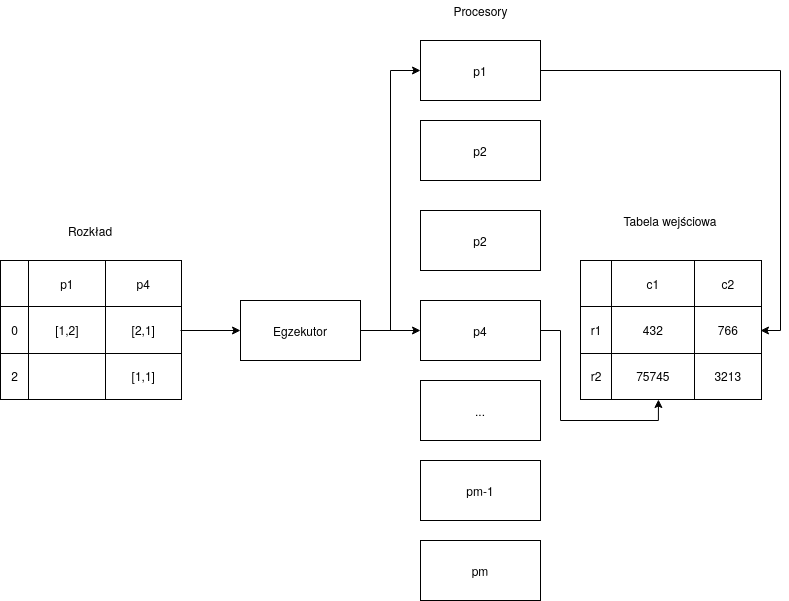
\includegraphics[width=.8\hsize]{fig/executor.png}
\caption{Schemat działania egzekutora\label{diag:executor}}
\source{Opracowanie własne}
\end{figure}
\medskip

Istnieje możliwość, w której oszacowanie czasu nie pokryło się z rzeczywistością. Sytuacja została szerzej opisana w rozdziale \ref{chap:extend}

Na diagramach \ref{diag:sched_20j420} i \ref{diag:sched_100j4m} przedstawione zostały wykresy Gantta dla przykładowych problemów.

\begin{figure}[!tbh]
\centering
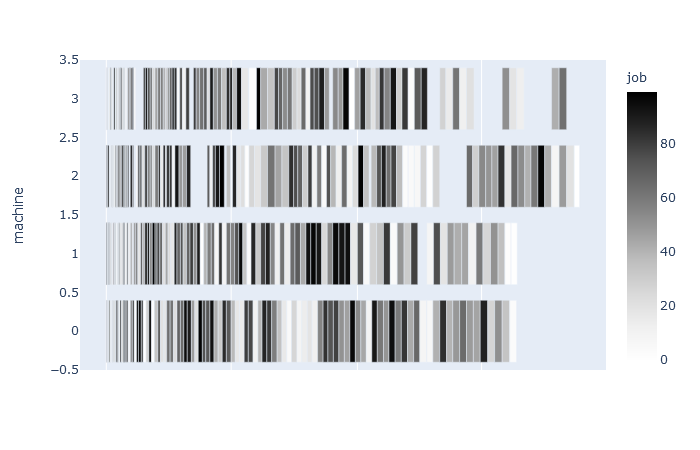
\includegraphics[width=.8\hsize]{fig/newplot_trim100j4m.png}
\caption{Przykładowe zaszeregowanie dla 100 zadań i 4 maszyn\label{diag:sched_100j4m}}
\source{Opracowanie własne}
\end{figure}
\medskip

\begin{figure}[!tbh]
\centering
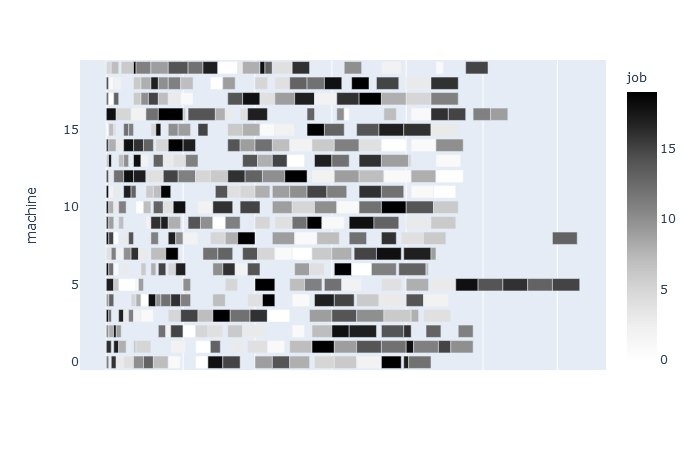
\includegraphics[width=.8\hsize]{fig/newplot_trim20j20m.png}
\caption{Przykładowe zaszeregowanie dla 20 zadań i 20 maszyn\label{diag:sched_20j420}}
\source{Opracowanie własne}
\end{figure}
\medskip

\chapter{Analiza sprawności dyspozytora}

W celu analizy sprawności dyspozytora przeprowadzono serie testów.
Testy różniły się między sobą
\begin{enumerate}
    \item ilością kolumn
    \item ilością wierszy
    \item czasem wykonywania poszczególnych operacji
    \item grafem konfliktu
\end{enumerate}

Wyniki testów dla algorytmu \emph{INSERTION WITH BEAM SEARCH} określają potencjalne jego zastosowania. Są to albo zbiory danych, gdzie ilości wierszy i kolumn po zgrupowaniu są bardzo małe (na przykład kilkadziesiąt wierszy i kilka kolumn), albo operacje, których naiwne zrównoleglanie trwa bardzo długo (wiele godzin). Naturalnie istnieje wiele takich przypadków, gdzie pożądanym jest sprowadzenie poprzez grupowanie dużych ilości wierszy do niewielu grup, lub operacji, których czas wykonania jest liczony w dniach. Na wykresach \ref{diag:relplot_128j} i \ref{diag:relplot_16m} znajdują się wykresy czasów wykonania operacji w zależności od, odpowiednio, ilości maszyn i ilości zadań.

\begin{figure}[!tbh]
\centering
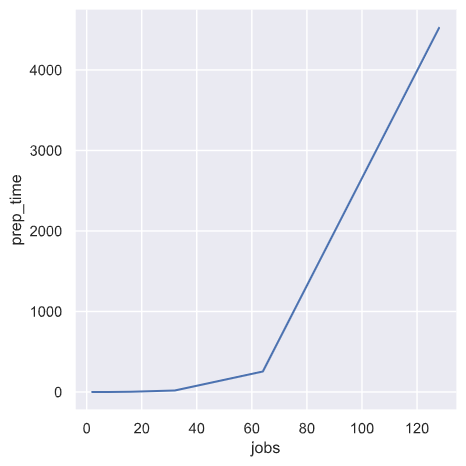
\includegraphics[width=.8\hsize]{fig/relplot_128j.png}
\caption{Porównanie czasu przygotowania operacji dla 128 operacji w zależności od ilości maszyn\label{diag:relplot_128j}}
\source{Opracowanie własne}
\end{figure}\medskip

\begin{figure}[!tbh]
\centering
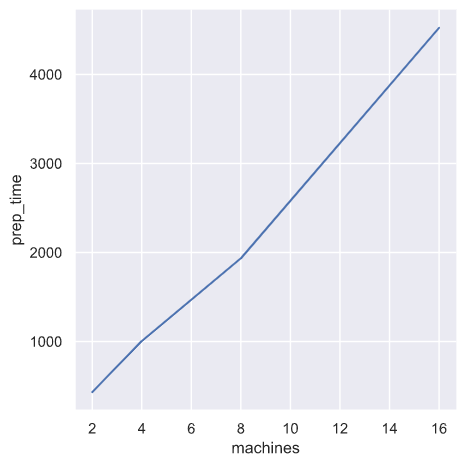
\includegraphics[width=.8\hsize]{fig/relplot_16m.png}
\caption{Porównanie czasu przygotowania operacji dla 16 maszyn w zależności od ilości zadań\label{diag:relplot_16m}}
\source{Opracowanie własne}
\end{figure}\medskip

\chapter{Analiza sprawności algorytmów dla podproblemu}

W celu analizy sprawności algorytmu \emph{INSERTION WITH BEAM SEARCH} porównano sumę czasów działania dyspozytora oraz wykonywania zaszeregowania z sekwencyjnym czasem wykonywania operacji dla tych samych danych.

\chapter{Potencjalne kierunki rozwoju pracy} \label{chap:extend}

Praca otwiera kilka tematów, o które może być rozszerzona oraz kilka potencjalnych tematów nowych prac.
\medskip

W celu pełnego wprowadzenia systemu do użycia, należy rozwiązać problem potencjalnych różnic pomiędzy założonym czasem operacji a czasem rzeczywistym. System obecnie stosuje margines bezpieczeństwa (niewielką wartość dodaną do szacowanego czasu operacji).
W pełni rozwinięty system powinien mieć tolerancję na takie błędy i wprowadzać korekty do rozkładu w trakcie jego wykonywania.
\medskip

Jako całkiem nowy temat, wartościowym byłoby poddanie analizie prawdopodobnie częściej spotykanego przypadku pominięcia grafu konfliktu, czyli zaimplementowania systemu dla modelu \emph{Multiprocessor Open Shop Schedule}.
\medskip

Kolejnym tematem, który został zauważony w trakcie analizy zagadnienia są szczególne (a zarazem najczęstsze) przypadki \emph{PCOSS} gdy graf konfliktu sprowadza się do grafu konfliktu wyłącznie dla kolumn, tj. z pominięciem krawędzi "pionowych" (między wierszami). Daje to potencjał do znalezienia i zastosowania bardziej optymalnych algorytmów.
\medskip

Zaproponowany system można zaimplementować jako tzw. \emph{scheduler}, na przykład w module \emph{Dask} języka \emph{Python}, który jest powszechnie stosowany przy zrównolegnianiu operacji na \emph{DataFrame-ach}.

% zakończenie
\summary

W pracy zaproponowano model systemu pozwalającego na redukcję czasu wykonywania serii operacji na danych tabelarycznych. System taki, prawdopodobnie z uwagi na specyficzną grupę odbiorców, nie został zaimplementowany w żadnym ze znanych modułów dostępnych w powszechnych językach programowania.
\medskip

Wybór problemu szeregowania zadań częściowo zależnych w systemie otwartym został podyktowany jego największą generalizacją spośród problemów typu powszechnych systemów szeregowania na maszynach dedykowanych. Jego ograniczanie do innych problemów nie powinno przynosić dużych wyzwań.
\medskip

Praca otwiera drogę do jej rozszerzenia, implementacji w komercyjnych produktach oraz optymalizacji.

% załączniki (opcjonalnie):
\appendix
\chapter{Tytuł załącznika jeden}

Treść załącznika jeden.

\chapter{Tytuł załącznika dwa}

Treść załącznika dwa.

% literatura (obowiązkowo):
\bibliographystyle{unsrt}
\bibliography{xml}

% spis tabel (jeżeli jest potrzebny):
\listoftables

% spis rysunków (jeżeli jest potrzebny):
\listoffigures

\oswiadczenie

\end{document}
